Construye un autómata finito en Octave:

\begin{enumerate}[a)]
  \item Abre el script de Octave fa.m y pruébalo con el ejemplo dado ( véase la ayuda del script ) en el repositorio de GitHub.

    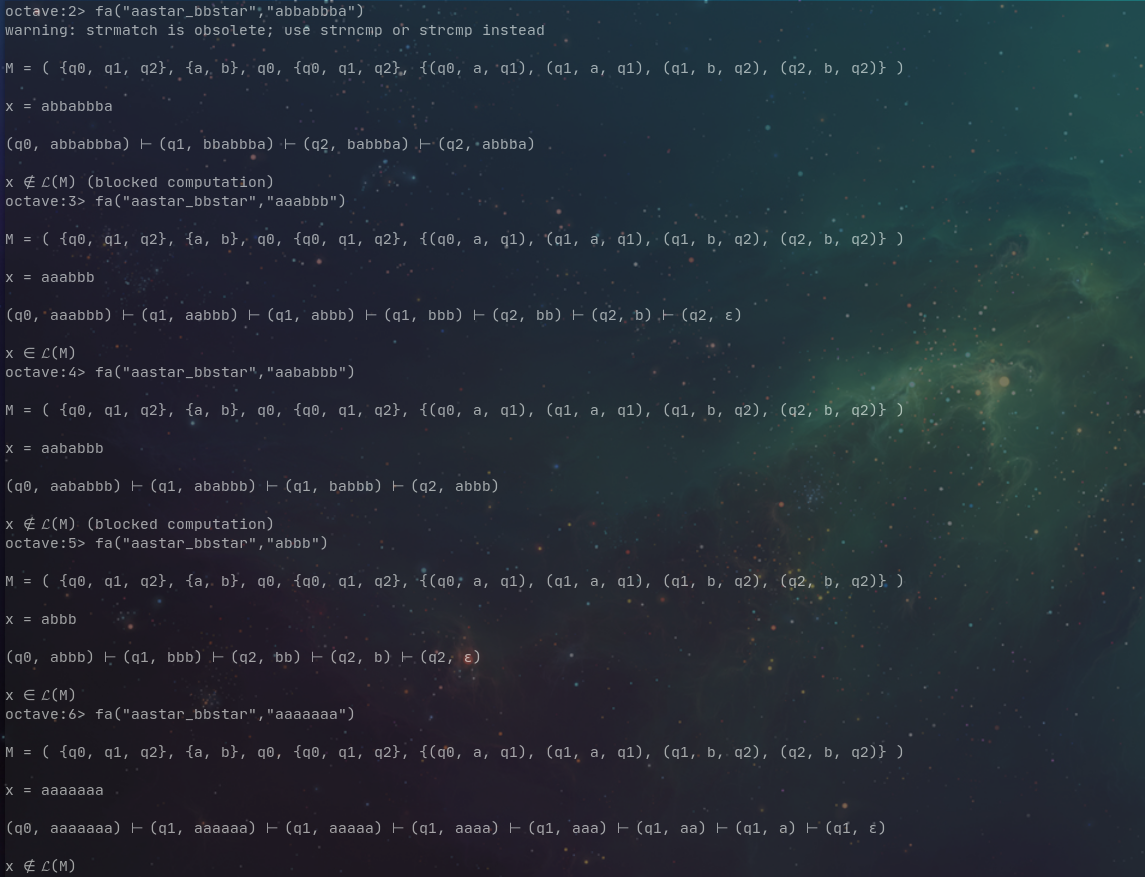
\includegraphics[width=0.85\textwidth]{images/octaveAutomataEjemplo.png}

  \item Crea un archivo JSON que describa el autómata creado en la actividad 1 y pruébalo.

    El archivo JSON que describe al autómata creado en la actividad 1 contiene lo siguiente:

    \begin{verbatim}
{
  "K" : ["q0", "q1", "q2"],
  "A" : ["a", "b"],
  "s" : "q0",
  "F" : ["q2"],
  "t" : [["q0", "a", "q2"],
         ["q0", "b", "q1"],
         ["q1", "a", "q1"],
         ["q1", "b", "q1"],
         ["q2", "a", "q1"],
         ["q2", "b", "q1"]]
}
    \end{verbatim}

    Uso del script fa.m con las 6 cadenas del ejercicio 1.2:

    %\includegraphics{}


\end{enumerate}
